\chapter{System Overview}

The proposed system is built around three main components: a camera module, a microcontroller-based processing unit, and a mobile application that serves as the user interface. These components are interconnected via a network to ensure seamless data flow. At the heart of the imaging system is the Arducam Mega 3MP camera, which communicates with the STM32L475 IoT Discovery Kit (DISCO\_L475\_IOT1) over an SPI interface. This microcontroller board leverages its onboard Wi-Fi to establish a connection with a remote TCP server, allowing real-time data transmission. Meanwhile, the mobile application provides a user-friendly interface to interact with the system. A high-level overview of the system’s hardware configuration is illustrated in Fig.~\ref{overall}.

\begin{figure}[h!]
  \centering
  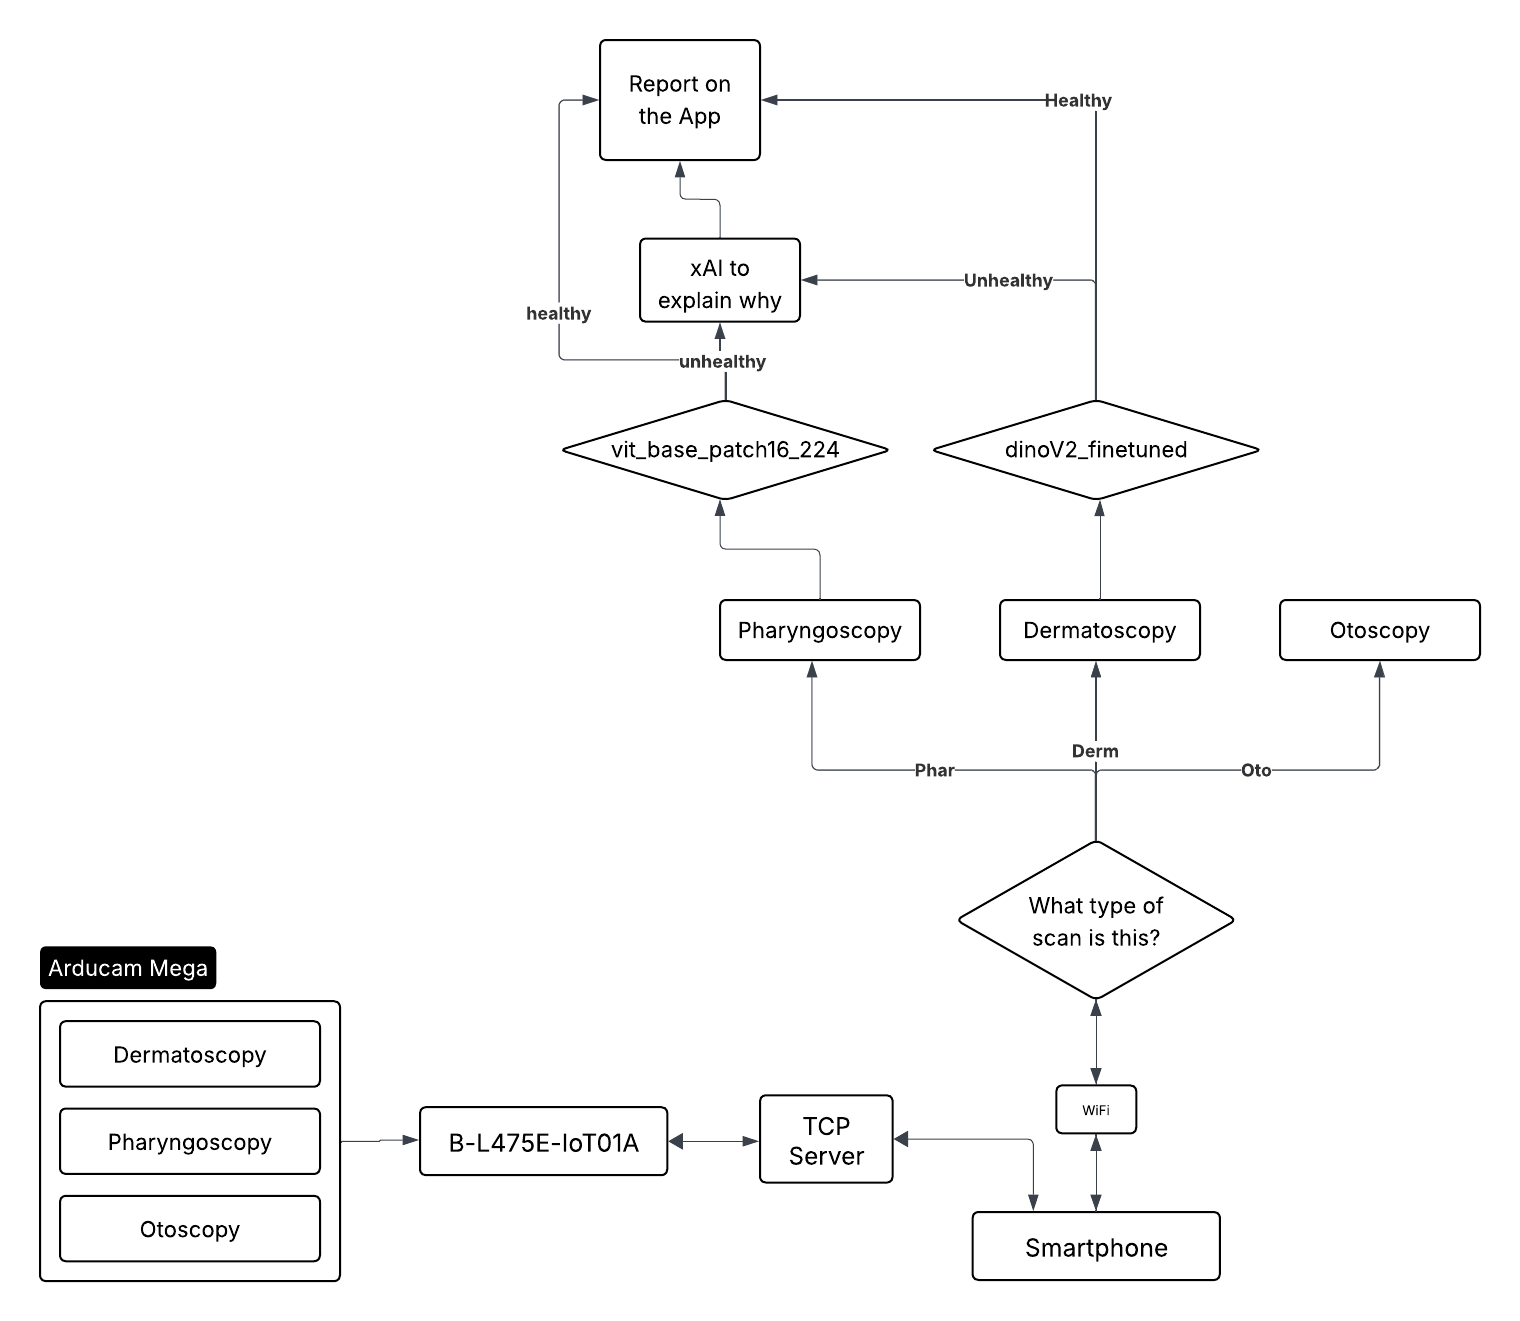
\includegraphics[width=0.8\linewidth]{system_diagram.png}
  \caption{Block diagram of the complete system.}
  \label{overall}
\end{figure}

\section{Camera Selection}

To ensure reliable image analysis using AI-based models, a resolution of at least 1080p is generally required. This level of detail is crucial for preserving fine visual features that AI algorithms rely on for tasks like classification, detection, or segmentation. While the Arducam Mega 3MP does not conform precisely to the 1920×1080 (1080p) specification, it supports a resolution of approximately 2048×1536, which comfortably exceeds the requirement. In addition to meeting resolution needs, the module offers a compact size and low power consumption, making it well-suited for embedded applications where space and energy efficiency are critical.

\section{Microcontroller Platform}

The STM32L475 IoT Discovery Kit was chosen for its low-power ARM Cortex-M4 microcontroller and the wide range of onboard sensors and communication modules, including Wi-Fi, Bluetooth, and NFC. This makes it an ideal platform for rapid prototyping of IoT applications. Its power efficiency is crucial for battery-powered or energy-constrained scenarios, and the board provides enough processing capability to handle real-time interfacing with the camera and network communication tasks.

\section{RTOS Selection: Zephyr}

Firmware development for the STM32L475 is carried out using the Zephyr RTOS, an open-source, real-time operating system tailored for embedded devices with limited resources. Zephyr offers vital functionalities like multithreading, hardware abstraction, and built-in networking stacks. These features are essential for coordinating tasks such as camera control, SPI-based communication, and managing the Wi-Fi module. One of Zephyr’s key strengths is its modularity, allowing developers to include only the components required for their specific application, keeping the firmware lightweight and efficient. The wide board support and active community also make Zephyr a robust choice for embedded development.

\section{Communication Protocol: TCP}

TCP was selected as the communication protocol between the microcontroller and the server due to its reliability. Unlike UDP, TCP provides guaranteed delivery, in-order packet transmission, and error checking, which are essential for transmitting critical data such as images and camera configuration commands. While TCP introduces slightly more overhead than UDP, its robustness outweighs this cost, especially in use cases where data integrity and reliable communication are paramount. The use of TCP ensures that image data is transmitted accurately to the server without loss or corruption.

